%% One-column to two-column: notitlepage -> twocolumn
\documentclass[pra,aps,notitlepage,superscriptaddress,showpacs,showkeys]{revtex4-1}
\usepackage{amsmath,amsthm,amssymb,graphicx,subfigure,tikz,xcolor}
\usepackage[unicode=true]{hyperref}
\usepackage{mathdots}
\usepackage{booktabs}
\usepackage{braket}
\usepackage{threeparttable}

\hypersetup{
     colorlinks=true,       		% false: boxed links; true: colored links
     linkcolor=blue,          	% color of internal links
     citecolor=red,            % color of links to bibliography
    % filecolor=blue,      		% color of file links
     urlcolor=magenta,           	% color of external links
    % runcolor=cyan
 }

%% THEOREMS -------------------------------------------------------
\newtheorem{theorem}{Theorem}
\newtheorem*{theorem*}{Theorem}
\newtheorem{corollary}{Corollary}
\newtheorem*{corollary*}{Corollary}
\newtheorem{lemma}{Lemma}
\newtheorem*{lemma*}{Lemma}
\newtheorem{proposition}{Proposition}
\newtheorem*{proposition*}{Proposition}
\theoremstyle{definition}
\newtheorem{definition}{Definition}
\newtheorem*{definition*}{Definition}
\theoremstyle{remark}
\newtheorem{remark}{Remark}
\newtheorem*{remark*}{Remark}
%% ----------------------------------------------------------------
\newcommand{\tr}{\mbox{tr}}

%% Supplementary Materials commands ----------------------------
\renewcommand{\thesection}{S\Roman{section}}
%\setcounter{section}{0}  %  this will re-count section from 1
\renewcommand{\theequation}{S\arabic{equation}}
%\setcounter{equation}{0}  %  this will re-count eq from 1
\renewcommand{\thefigure}{S\arabic{figure}}
%\setcounter{figure}{0}  %  this will re-count eq from 1

\begin{document}


\title{Supplemental Material for ``Experimental Demonstration of Quantum Contextuality beyond Bell Nonlocality''}


\author{Zheng-Hao Liu}
\affiliation{CAS Key Laboratory of Quantum Information, University of Science and Technology of China, Hefei 230026, People's Republic of China}
\affiliation{Synergetic Innovation Center of Quantum Information and Quantum Physics, University of Science and Technology of China, Hefei 230026, People's Republic of China}

\author{Hui-Xian Meng}
\affiliation{Theoretical Physics Division, Chern Institute of Mathematics, Nankai University, Tianjin 300071, People's Republic of China}

\author{Zhen-Peng Xu}
\affiliation{Naturwissenschaftlich-Technische Fakult\"{a}t, Universit\"{a}t Siegen, Walter-Flex-Stra{\ss}e 3, 57068 Siegen, Germany}

\author{Jie Zhou}
\affiliation{Theoretical Physics Division, Chern Institute of Mathematics, Nankai University, Tianjin 300071, People's Republic of China}


\author{Sheng Ye}
\affiliation{CAS Key Laboratory of Quantum Information, University of Science and Technology of China, Hefei 230026, People's Republic of China}
\affiliation{Synergetic Innovation Center of Quantum Information and Quantum Physics, University of Science and Technology of China, Hefei 230026, People's Republic of China}

\author{Qiang Li}
\affiliation{CAS Key Laboratory of Quantum Information, University of Science and Technology of China, Hefei 230026, People's Republic of China}
\affiliation{Synergetic Innovation Center of Quantum Information and Quantum Physics, University of Science and Technology of China, Hefei 230026, People's Republic of China}

\author{Kai Sun}
\affiliation{CAS Key Laboratory of Quantum Information, University of Science and Technology of China, Hefei 230026, People's Republic of China}
\affiliation{Synergetic Innovation Center of Quantum Information and Quantum Physics, University of Science and Technology of China, Hefei 230026, People's Republic of China}

\author{Hong-Yi Su}
\affiliation{Graduate School of China Academy of Engineering Physics, Beijing 100193, People's Republic of China}

\author{Ad\'{a}n Cabello}
\affiliation{Departamento de Fsica Aplicada II, Universidad de Sevilla, E-41012 Sevilla, Spain}


\author{Jing-Ling Chen}
%\email{chenjl@nankai.edu.cn}
\affiliation{Theoretical Physics Division, Chern Institute of Mathematics, Nankai University, Tianjin 300071, People's Republic of China}

\author{Jin-Shi Xu}
%\email{jsxu@ustc.edu.cn}
\affiliation{CAS Key Laboratory of Quantum Information, University of Science and Technology of China, Hefei 230026, People's Republic of China}
\affiliation{Synergetic Innovation Center of Quantum Information and Quantum Physics, University of Science and Technology of China, Hefei 230026, People's Republic of China}

\author{Chuan-Feng Li}
%\email{cfli@ustc.edu.cn}
\affiliation{CAS Key Laboratory of Quantum Information, University of Science and Technology of China, Hefei 230026, People's Republic of China}
\affiliation{Synergetic Innovation Center of Quantum Information and Quantum Physics, University of Science and Technology of China, Hefei 230026, People's Republic of China}

\author{Guang-Can Guo}
\affiliation{CAS Key Laboratory of Quantum Information, University of Science and Technology of China, Hefei 230026, People's Republic of China}
\affiliation{Synergetic Innovation Center of Quantum Information and Quantum Physics, University of Science and Technology of China, Hefei 230026, People's Republic of China}


%\pacs{03.65.Ud, 03.67.Mn, 42.50.Xa}

\maketitle


\section{The theoretical part}


\subsection{The Bell inequality and noncontextual inequality associated with $I_{3322}^{\rm CSW}$}
The symmetric version of the inequality $I_{3322}\le 0$ proposed in Ref.~\cite{BG08} is
\begin{equation}
 I_{3322} \stackrel{\mbox{\tiny{LHV}}}{\leq} 0.
\end{equation}
with
\begin{eqnarray}
 I_{3322} &=&P(0,0 \vert 0,1) + P(0,0 \vert 0,2) + P(0,0 \vert 1,0)+ P(0,0 \vert 1,2) + P(0,0 \vert 2,0) + P(0,0 \vert 2,1) \nonumber \\
                    &&- P(0,0 \vert 1,1) - P(0,0 \vert 2,2) - P(0,\_ \vert 0,\_) - P(0,\_ \vert 1,\_) - P(\_,0 \vert \_,0) - P(\_,0 \vert \_,1).
                    \label{I3322BG}
\end{eqnarray}
Using the equation
\begin{equation}
-P(A_x=a,B_x=b)=-1+\sum_{(a',b') \neq (a,b)} P(A_x=a',B_y=b')
\label{transformations}
\end{equation}
to replace probabilities with minus signs by the corresponding positive probabilities, we obtain
\begin{equation}
 I_{3322} = I_{3322}^{\rm CSW} - 6,
\end{equation}
where
\begin{eqnarray}
 I_{3322}^{\rm CSW}
 &=&P(0,0 \vert 0,1) + P(0,0 \vert 0,2) + P(0,0 \vert 1,0)+ P(0,0 \vert 1,2) + P(0,0 \vert 2,0) + P(0,0 \vert 2,1) \nonumber \\
 &&+ P(0,1 \vert 1,1) + P(1,0 \vert 1,1) + P(1,1 \vert 1,1)+ P(0,1 \vert 2,2) + P(1,0 \vert 2,2) + P(1,1 \vert 2,2) \nonumber \\
 &&+ P(1,\_ \vert 0,\_) +P(1,\_ \vert 1,\_) + P(\_,1 \vert \_,0) + P(\_,1 \vert \_,1).
\label{I3322CSW}
\end{eqnarray}
Therefore, the inequality $I_{3322}\le 0$ can be written as
\begin{equation}
 I_{3322}^{\rm CSW} \stackrel{\mbox{\tiny{LHV}}}{\leq} 6.\label{i3322}
\end{equation}
The maximal Bell nonlocality (BN) of inequality \eqref{i3322} for two qubits is exactly $ I_{3322}^{\rm BN}=6.25$, which can be  obtained in the following case:
\begin{eqnarray}
\left\{
  \begin{array}{ll}
    A_0=B_0=\left(
          \begin{array}{cc}
            \frac{\sqrt{2-\sqrt{3}}}{2} & \frac{\sqrt{2+\sqrt{3}}}{2} \\
            \frac{\sqrt{2+\sqrt{3}}}{2} & \frac{\sqrt{2}-\sqrt{6}}{4} \\
          \end{array}
        \right),
    A_1=B_2=\left(
          \begin{array}{cc}
            \frac{\sqrt{2+\sqrt{3}}}{2} & \frac{\sqrt{2-\sqrt{3}}}{2} \\
            \frac{\sqrt{2-\sqrt{3}}}{2} & -\frac{\sqrt{2+\sqrt{3}}}{2} \\
          \end{array}
        \right),
    A_2=B_1=\left(
          \begin{array}{cc}
            -\frac{1}{\sqrt{2}} & \frac{1}{\sqrt{2}} \\
            \frac{1}{\sqrt{2}} & \frac{1}{\sqrt{2}} \\
          \end{array}
        \right), & \\
\rho=\frac{1}{2}\left(
       \begin{array}{cccc}
        1 & 0 & 0 & 1 \\
         0 & 0 & 0 & 0 \\
         0 & 0 & 0 & 0 \\
         1 & 0 & 0 & 1 \\
       \end{array}
     \right)=\ket{\Phi^+}\langle\Phi^+|
,\ket{\Phi^+}=(|00\rangle+|11\rangle)/\sqrt{2}, &\\
P(a,b|i,j)={\rm{Tr}}\left[\frac{I_2+(-1)^aA_i}{2}\otimes \frac{I_2+(-1)^bB_j}{2}\rho\right]. &
  \end{array}
\right.
\end{eqnarray}



For the exclusivity graph $G$ (Fig.1 in the main text) associated with $I_{3322}^{\rm CSW}$,
a noncontextual (NC) inequality is constructed with the form
\begin{eqnarray}
I_{3322}^{\rm CSW}
=\sum_{i\in V}P_{|\psi\rangle}(A_i=1)-\sum_{(i,j)\in E}P_{|\psi\rangle}(A_i=1,A_j=1)\overset{{\rm{NCHV}}}\leq& 6,
\label{I3322QC}
\end{eqnarray}
where $V$ and $E$, respectively, denote the vertex and edge sets of graph $G$,
$P_{|\psi\rangle}(A_i=1)$ denotes the probability of obtaining result 1 when the observable $|A_i\rangle\langle A_i|$ is measured on the state $|\psi\rangle $,  i.e., $P_{|\psi\rangle}(A_i=1)= |\langle \psi|A_i\rangle|^2,$ $P_{|\psi\rangle}(A_i=1,A_j=1)$, i.e.,  $P_{|\psi\rangle}(A_i=1)P_{|A_i\rangle}(A_j=1)$, represents experimental imprecision of $|A_i\rangle\bot |A_j\rangle$ when vertex $i$ and vertex $j$ are connected in the graph.

The optimal quantum contextuality (QC) of inequality \eqref{I3322QC} is just the Lov\'asz number of $G$, i.e.,  $I_{3322}^{\rm QC}=\vartheta(G)\approx6.58841287$, which is obtained in the
five-dimensional quantum system. In Table. \ref{numerical}, we list
the optimal settings and the optimal state numerically.
\begin{table}[t]
\centering
\caption{Numerically optimal settings and optimal state in a five-dimensional system for for $I_{3322}^{\rm QC}\approx6.58841287$.}
  \begin{tabular}{lccccc} \hline \hline
$|A_i\rangle$ & $i_1$ & $i_2$ & $i_3$ & $i_4$ & $i_5$ \\
\hline
$|A_1\rangle$  & $0$ & $0$ & $0$ & $0$ & $1$ \\
$|A_2\rangle$  & $0.538648$ & $-0.458664$ & $0.0322917$ & $-0.706005$ & $0$ \\
$|A_3\rangle$  & $0.672155$ & $-0.188775$ & $-0.359722$ & $0.619009$ & $0$ \\
$|A_4\rangle$  & $0$ & $0.95651$ & $0$ & $0.2917$ & $0$ \\
$|A_5\rangle$  & $0.188775$ & $-0.672155$ & $-0.359722$ & $-0.619009$ & $0$ \\
$|A_6\rangle$  & $0.192831$ & $-0.671551$ & $-0.44115$ & $0.563224$ & $0$ \\
$|A_7\rangle$  & $0.912455$ & $0$ & $-0.409176$ & $0$ & $0$ \\
$|A_8\rangle$  & $-0.946087$ & $0$ & $0$ & $0.323911$ & $0$ \\
$|A_9\rangle$  & $0$ & $1$ & $0$ & $0$ & $0$ \\
$|A_{10}\rangle$ & $1$ & $0$ & $0$ & $0$ & $0$ \\
$|A_{11}\rangle$ & $0$ & $0.912455$ & $0.409176$ & $0$ & $0$ \\
$|A_{12}\rangle$ & $0.95651$ & $0$ & $0$ & $0.2917$ & $0$ \\
$|A_{13}\rangle$ & $0$ & $0$ & $1$ & $0$ & $0$ \\
$|A_{14}\rangle$ & $0$ & $-0.946087$ & $0$ & $0.323911$ & $0$ \\
$|A_{15}\rangle$ & $-0.671551$ & $0.192831$ & $0.44115$ & $0.563224$ & $0$ \\
$|A_{16}\rangle$ & $-0.458664$ & $0.538648$ & $-0.0322917$ & $-0.706005$ & $0$ \\
\hline
$|\psi\rangle$ & $-0.674033$ & $0.674033$ & $0.302255$ & $0$ & $0$\\
  \hline \hline
   \end{tabular}
\label{numerical}
\end{table}
%%-----------------------------------------------------%%
\begin{remark}
If we take the following analytical settings and state in Table. \ref{analytical}, then  the maximal quantum contextuality  is
\[
I_{3322}^{\rm CSW} = \sum_{i=1}^{16} |\langle \psi|i\rangle|^2 -0= (355+209\cos(2\tau)+112\sin(2\tau))/90,
\]
whose maximal point is $\tau = \arctan[(-209 + 5 \sqrt{2249})/112]$ with the maximum $\left(71+\sqrt{2249}\right)/18 \approx 6.57909$.
And if we choose $\tau = 2\pi/25$, then $\sum_{i=1}^{16} |\langle \psi|i\rangle|^2 \approx 6.57894$. It's easy to see that this numerical contextuality is close to the optimal one with an error $0.0014$.
\begin{table}[t]
\centering
\caption{An analytical settings and state in a five-dimensional system for $I_{3322}^{\rm CSW}$.}
  \begin{tabular}{lccccc} \hline \hline
$|A_i\rangle$ & $i_1$ & $i_2$ & $i_3$ & $i_4$ & $i_5$ \\
\hline
$|A_1\rangle$  & $0$ & $0$ & $0$ & $0$ & $1$ \\
$|A_2\rangle$  & $\frac{1}{2}$ & $\frac{1}{2}$ & $0$ & $-\frac{1}{\sqrt{2}}$ & $0$ \\
$|A_3\rangle$  & $\frac{3}{2 \sqrt{5}}$ & $\frac{1}{2 \sqrt{5}}$ & $\frac{1}{\sqrt{10}}$ & $\sqrt{\frac{2}{5}}$ & $0$ \\
$|A_4\rangle$  & $0$ & $\frac{2 \sqrt{2}}{3}$ & $0$ & $-\frac{1}{3}$ & $0$ \\
$|A_5\rangle$  & $\frac{1}{2 \sqrt{5}}$ & $\frac{3}{2 \sqrt{5}}$ & $\frac{1}{\sqrt{10}}$ & $-\sqrt{\frac{2}{5}}$ & $0$ \\
$|A_6\rangle$  & $\frac{1}{2 \sqrt{5}}$ & $\frac{3}{2 \sqrt{5}}$ & $\frac{1}{\sqrt{10}}$ & $\sqrt{\frac{2}{5}}$ & $0$ \\
$|A_7\rangle$  & $\frac{2 \sqrt{2}}{3}$ & $0$ & $\frac{1}{3}$ & $0$ & $0$ \\
$|A_8\rangle$  & $\frac{2 \sqrt{2}}{3}$ & $0$ & $0$ & $-\frac{1}{3}$ & $0$ \\
$|A_9\rangle$  & $0$ & $1$ & $0$ & $0$ & $0$ \\
$|A_{10}\rangle$ & $1$ & $0$ & $0$ & $0$ & $0$ \\
$|A_{11}\rangle$ & $0$ & $\frac{2 \sqrt{2}}{3}$ & $\frac{1}{3}$ & $0$ & $0$ \\
$|A_{12}\rangle$ & $\frac{2 \sqrt{2}}{3}$ & $0$ & $0$ & $\frac{1}{3}$ & $0$ \\
$|A_{13}\rangle$ & $0$ & $0$ & $1$ & $0$ & $0$ \\
$|A_{14}\rangle$ & $0$ & $\frac{2 \sqrt{2}}{3}$ & $0$ & $\frac{1}{3}$ & $0$ \\
$|A_{15}\rangle$ & $\frac{3}{2 \sqrt{5}}$ & $\frac{1}{2 \sqrt{5}}$ & $\frac{1}{\sqrt{10}}$ & $-\sqrt{\frac{2}{5}}$ & $0$  \\
$|A_{16}\rangle$ & $\frac{1}{2}$ & $\frac{1}{2}$ & $0$ & $\frac{1}{\sqrt{2}}$ & $0$ \\
\hline
$|\psi\rangle$ & $\frac{\cos\tau}{\sqrt{2}}$ & $\frac{\cos\tau}{\sqrt{2}}$ & $\sin\tau$ & $0$ & $0$ \\
  \hline \hline
   \end{tabular}
\label{analytical}
\end{table}
\end{remark}


\subsection{QC of $I_{3322}^{\rm CSW}$ in a four-dimensional system}




 In the four-dimensional quantum system, take
\begin{eqnarray}
\left\{
  \begin{array}{ll}
    |\psi\rangle=[\cos{[\theta]},\sin{[\theta]}\cos{[\phi]},
\sin{[\theta]}\sin{[\phi]}\cos{[\tau]},
\sin{[\theta]}\sin{[\phi]}\sin{[\tau]}] \\
    |A_i\rangle=[\cos{[\theta_i]},\sin{[\theta_i]}\cos{[\phi_i]},
\sin{[\theta_i]}\sin{[\phi_i]}\cos{[\tau_i]},
\sin{[\theta_i]}\sin{[\phi_i]}\sin{[\tau_i]}],
  \end{array}
\right.
\end{eqnarray}
for $i=1,2,\cdots, 16$. Then
\begin{widetext}
\begin{eqnarray}
\begin{split}
&~~~~P_{|\psi\rangle}(A_i=1)\\
&= |\langle \psi|A_i\rangle|^2\\
&=(\cos{[\theta]}\cos{[\theta_i]}+\sin{[\theta]}\sin{[\theta_i]}(\cos{[\phi]}\cos{[\phi_i]}
+\sin{[\phi]}\sin{[\phi_i]}(\cos{[\tau]}\cos{[\tau_i]}+\sin{[\tau]}\sin{[\tau_i]})))^2
\end{split}
\end{eqnarray}
\end{widetext} and
\begin{eqnarray}
\label{max}
\max\{I_{3322}^{\rm CSW}:\theta,\phi,\tau,\theta_i,\phi_i,\tau_i\}\approx 6.57152.
\end{eqnarray}
\begin{table}[t]
\centering
 \caption{Settings and state in a four-dimension system for $I_{3322}^{\rm CSW}$.}
 \begin{tabular}{lcccc} \hline \hline
$|A_i\rangle$ & $i_1$ & $i_2$ & $i_3$ & $i_4$  \\
\hline
$|A_1\rangle$  & $0$ & $0$ & $1$ & $0$  \\
$|A_2\rangle$  & $\cos{[\phi_1]}\cos{[\phi_2]}\ \ $ & $\sin{[\phi_1]}$ & $0$ & $-\cos{[\phi_1]}\sin{[\phi_2]}$\\
$|A_3\rangle$  & $\cos{[\phi_3]}$ & $\cos{[\phi_4]}\sin{[\phi_3]}$ & $0$ & $\sin{[\phi_3]}\sin{[\phi_4]}$ \\
$|A_4\rangle$  & $0$ & $\sin{[\phi_4]}$ & $0$ & $-\cos{[\phi_4]}$ \\
$|A_5\rangle$  & $\cos{[\phi_4]}\sin{[\phi_3]}$ & $\cos{[\phi_3]}$ & $0$ & $-\sin{[\phi_3]}\sin{[\phi_4]}$ \\
$|A_6\rangle$  & $\cos{[\phi_4]}\cos{[\phi_5]}$ & $\sin{[\phi_5]}$ & $0$ & $\cos{[\phi_5]}\sin{[\phi_4]}$ \\
$|A_7\rangle$  & $1$ & $0$ & $0$ & $0$ \\
$|A_8\rangle$  & $\sin{[\phi_4]}$ & $0$ & $0$ & $-\cos{[\phi_4]}$  \\
$|A_9\rangle$  & $0$ & $1$ & $0$ & $0$  \\
$|A_{10}\rangle$ & $1$ & $0$ & $0$ & $0$  \\
$|A_{11}\rangle$ & $0$ & $1$ & $0$ & $0$  \\
$|A_{12}\rangle$ & $\sin{[\phi_4]}$ & $0$ & $0$ & $\cos{[\phi_4]}$  \\
$|A_{13}\rangle$ & $0$ & $0$ & $1$ & $0$ \\
$|A_{14}\rangle$ & $0$ & $\sin{[\phi_4]}$ & $0$ & $\cos{[\phi_4]}$  \\
$|A_{15}\rangle$ & $\sin{[\phi_5]}$ & $\cos{[\phi_4]}\cos{[\phi_5]}$ & $0$ & $-\cos{[\phi_5]}\sin{[\phi_4]}$  \\
$|A_{16}\rangle$ & $\sin{[\phi_1]}$ & $\cos{[\phi_1]}\cos{[\phi_2]}$ & $0$ & $\cos{[\phi_1]}\sin{[\phi_2]}$  \\
\hline
$|\psi\rangle$ & $\frac{1}{\sqrt{2}}$ & $\frac{1}{\sqrt{2}}$ & $0$ & $0$\\
  \hline \hline
   \end{tabular}
\label{four-dimension}
\end{table}

To obtain Eq. (\ref{max}), it is sufficient to assume the settings and state have the form in Table \ref{four-dimension}, and the angles are sa follows:
\begin{widetext}
\begin{eqnarray}
\left\{
  \begin{array}{ll}
    \phi_{2}\approx 1.0156029707166405,\phi_{4}\approx 1.1802538214743192,\\
    \phi_{3}=\arctan{\frac{2\cos{\phi_4}}{\sin^2{\phi_4}}},
\phi_{1}=-\arctan{\frac{\cos{\phi_2}\cos{\phi_3}-\sin{\phi_2}\sin{\phi_3}\sin{\phi_4}}{\cos{\phi_4}\sin{\phi_3}}},
\phi_{5}=-\arctan{\frac{\cos{\phi_1}\cos{\phi_2+\phi_4}}{\sin{\phi_1}}}.
\end{array}
\right.
\end{eqnarray}
\end{widetext}
In this case, Table~\ref{four-dimension} becomes the following Table~\ref{four-dimension-b}.

\begin{table}[t]
\caption{Numerically optimal measurement settings and state in a four-dimension system for $I_{3322}^{\rm QC}\approx6.57152$.}
\label{numerica3}
\centering
%\begin{ruledtabular}
  \begin{tabular}{lccccc} 
  \hline \hline
$|A_i\rangle$ & $i_1$ & $i_2$ & $i_3$ & $i_4$  \\
\hline
$|A_1\rangle$ & $0$ & $0$ & $1$ & $0$  \\
$|A_2\rangle$  & $0.469723$ & $0.453743$ & $0$ & $0.757283$  \\
$|A_3\rangle$ & $0.746839$ & $0.253161$ & $0$ & $0.614931$  \\
$|A_4\rangle$  & $0$ & $0.924703$ & $0$ & $-0.38069$  \\
$|A_5\rangle$ & $0.253161$ & $0.746839$ & $0$ & $-0.614931$  \\
$|A_6\rangle$ & $0.249899$ & $0.754381$ & $0$ & $0.607009$  \\
$|A_7\rangle$ & $1$ & $0$ & $0$ & $0$  \\
$|A_8\rangle$  & $0.924703$ & $0$ & $0$ & $-0.38069$  \\
$|A_9\rangle$  & $0$ & $1$ & $0$ & $0$  \\
$|A_{10}\rangle$  & $1$ & $0$ & $0$ & $0$ \\
$|A_{11}\rangle$ & $0$ & $1$ & $0$ & $0$  \\
$|A_{12}\rangle$  & $0.924703$ & $0$ & $0$ & $0.38069$  \\
$|A_{13}\rangle$  & $0$ & $0$ & $1$ & $0$  \\
$|A_{14}\rangle$  & $0$ & $0.924703$ & $0$ & $0.38069$  \\
$|A_{15}\rangle$ & $0.754381$ & $0.249899$ & $0$ & $-0.607009$  \\
$|A_{16}\rangle$  & $0.453743$ & $0.469723$ & $0$ & $0.757283$  \\
\hline
$|\psi\rangle$ & $\frac{1}{\sqrt{2}}$ & $\frac{1}{\sqrt{2}}$ & $0$ & $0$\\
 \hline \hline
   \end{tabular}
%\end{ruledtabular}
\label{four-dimension-b}
\end{table}


In experiment, one can choose $\phi_{2}= 1.015,\phi_{4}= 1.180$, then the orthogonal relationship can be satisfied with errors $10^{-32}$, i.e.,
$$\sum_{(i,j)\in E}P_{|\psi\rangle}(A_i=1,A_j=1)\approx 9.62965\times 10^{-33}<10^{-32},$$
and $\max I_{3322}^{\rm CSW}\approx 6.57152.$



\begin{remark}
In fact, for $\phi_{2}= \pi/3,\phi_{4}=7\pi/18$, we can obtain that the orthogonal relationship is strictly satisfied  $(\sum_{(i,j)\in E}P_{|\psi\rangle}(A_i=1,A_j=1)=0)$ and $\max I_{3322}^{\rm CSW}\approx 6.56233.$
\end{remark}

\section{The experimental part}

\subparagraph{Testing experimental reliability of orbital angular momentum (OAM) qudit.} 
The two experimental tests rely on photonic polarization qubit and OAM qudit, and for the latter one it is vital to confirm that the measurements performed in experiment ideally represents the terms in~(\ref{I3322QC}).
Due to the complexity of a four-dimensional system, we opted out of a complete state tomography and, instead, chose to test the orthonormality of the 6 sets of complete bases used in our experiment. 

The Born rule declares that, for an observable corresponding to a self-adjoint operator $A$, the probability of obtaining result $\lambda_i$ on state $\ket{\psi}$ be $\braket{\psi|\Pi_i|\psi}$, where $\Pi_i$ is the projection operator onto the eigenspace of $A$ corresponding to the eigenvalue of $\lambda_i$. 
It follows immediately from the Born rule that when we prepare an eigenstate of $\Pi_i$, the probability of getting $\lambda_i$ in the measurement $A$ is $1$, while the probability of getting other $\lambda_{j\neq i}$s are $0$. 
For an ideal measurement, the complete set of bases should then be orthonormal, regardless of the exact bases settings we choose. 
Fig.~\ref{fig:exp-res-1} shows the result of testing orthonormality of the six sets of complete bases. When we prepared the state corresponding to one specific outcome, and then measured the corresponding projector, we (almost) always obtained that certain outcome.
Since the projectors to orthogonal bases commute with each other, the null counting rates between orthogonal states and projectors can also serve as proof of non-disturbance of compatible measurements. 
We thus infer that the measurements performed in the experiment are overall approximately ideal, and the data is suitable to be analyzed in the CSW framework using~(\ref{I3322QC}).


 \begin{figure}[t]
     \centering
     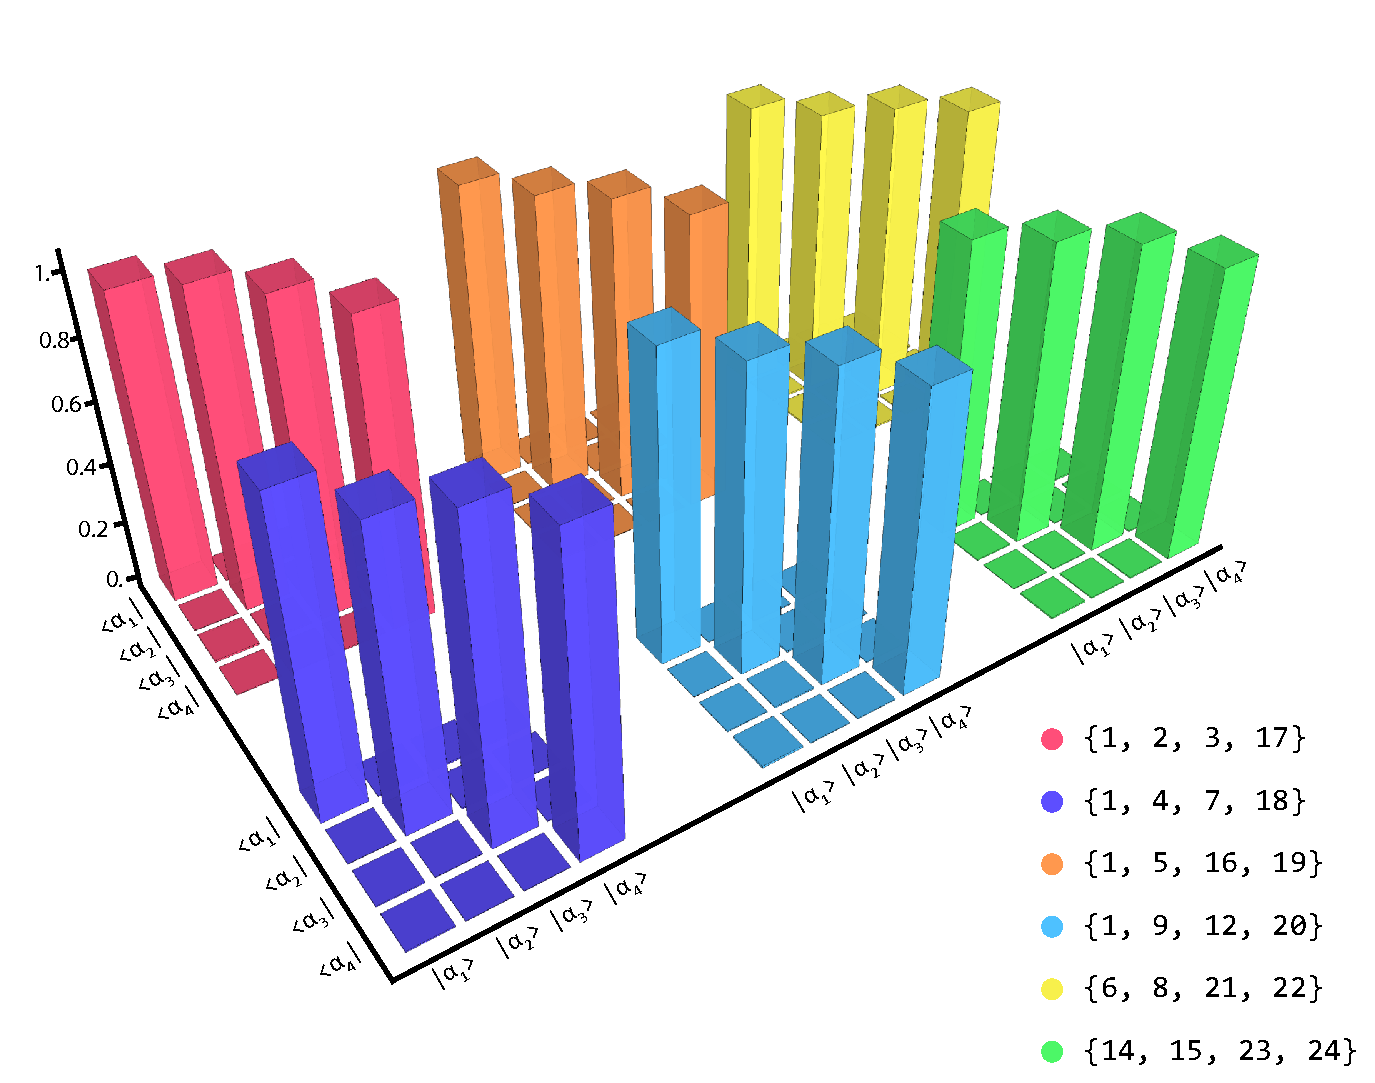
\includegraphics[width = .53\columnwidth] {fig/exp-res-1.pdf}
     \caption{Testing the orthonormality of the six sets of complete measurements used in the experiment, by enumerating detection probability between bases within each set.}
     \label{fig:exp-res-1}
 \end{figure}

 \subparagraph{Details about the single photon source.}
 The sample used in this experiment was a $2\mu m$ thick magnesium (Mg)-doped gallium nitride (GaN) film on 2 mm undoped GaN layer grown on sapphire substrate.
 This kind of sample was reported in~\cite{qli18s} and we followed their practice to pretreat the sample with acetone and isopropanol (1:1) solution and clean in ultrasound bath.
 The defects distributed over the sample surface, and a confocal microscopy system was exploited to excite the sample and collect emitted single photons.

 In our experiment, a 532 nm continuous wave laser was used to excite the GaN sample. The laser was reflected by a dichroic mirror, focused onto the sample by an objective lens with high numeric aperture of $1.25$. The fluorescence was collected by the same objective and filtered by the dichroic mirror and the band-pass filter.

 To examine attributes of the photoluminescence (PL) signal, it was coupled to a single mode fiber, and either guided to a SPAD for photon counting and spectrum measurement (band-pass filter was removed for this measurement), or a HBT interferometer setup for single photon verification.

 \begin{figure}[t]
     \centering
     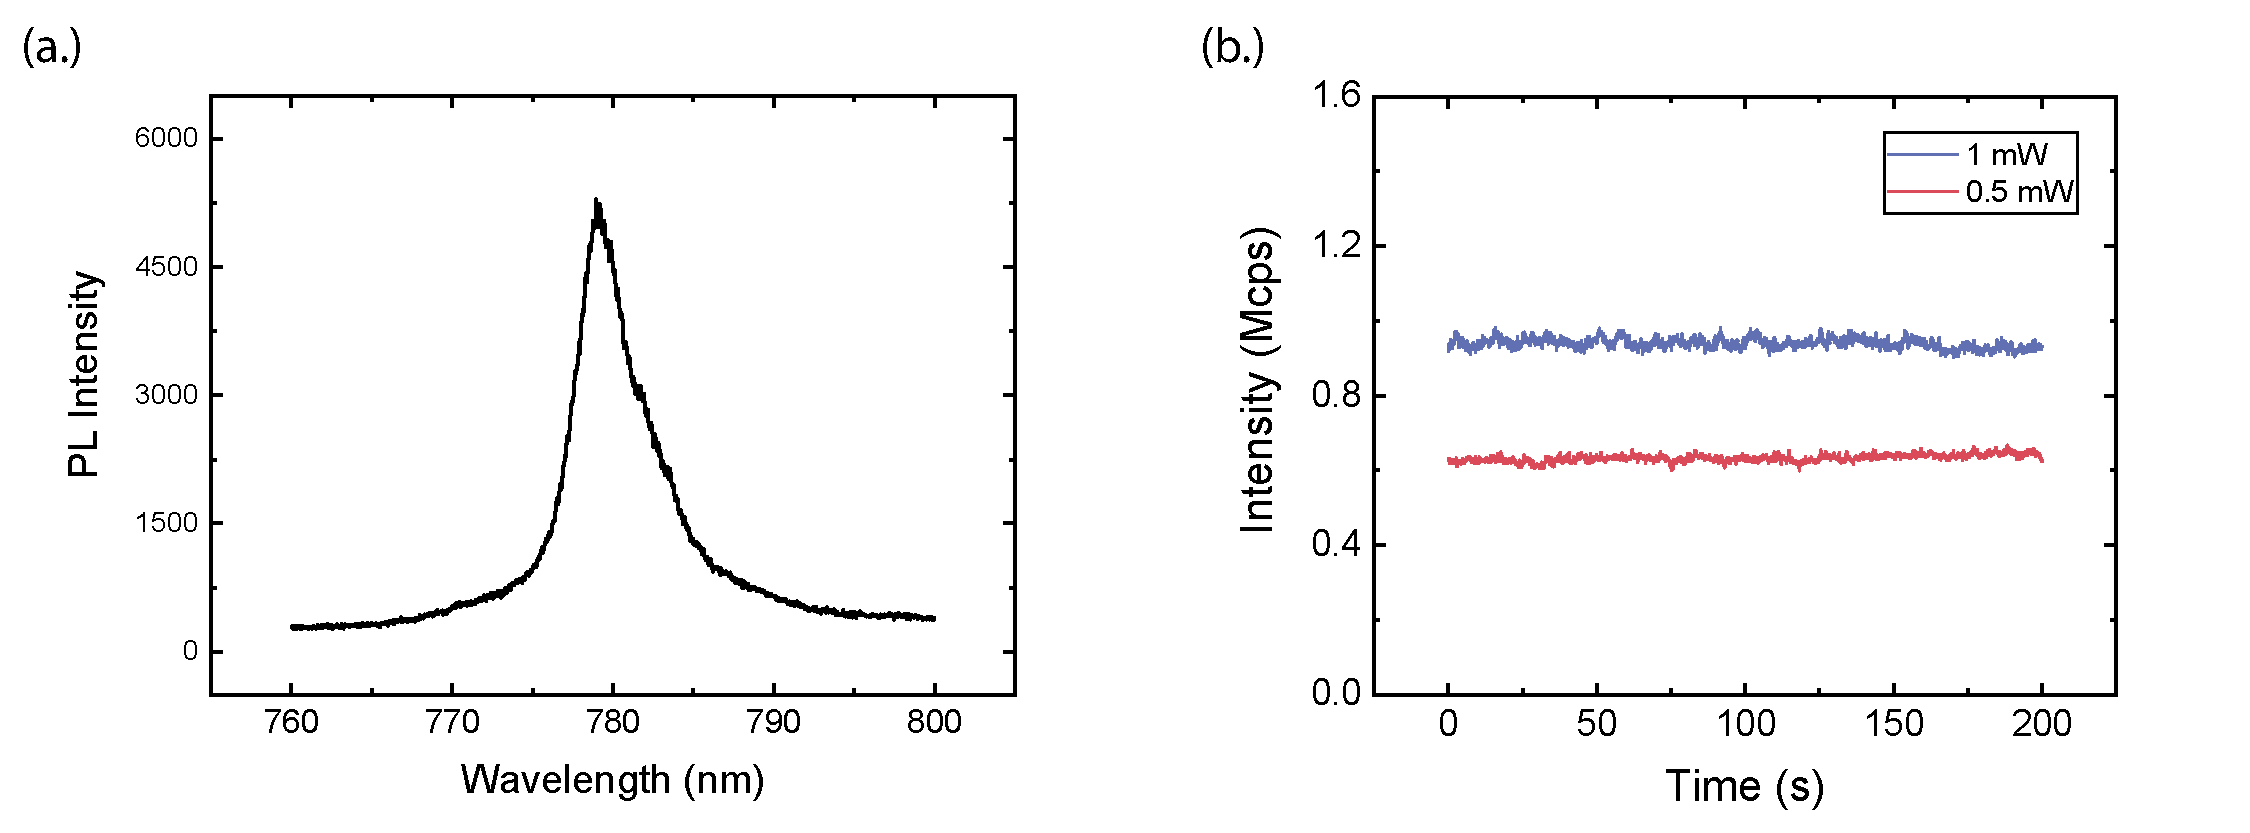
\includegraphics[width = .96 \linewidth]{fig/exp-sauce.pdf}
     \caption{The properties of the single photon source used in the contextuality experiment. (a.) the spectrum. The central wavelength of the emitter was $779.61nm$ and the FWHM was $4.97nm$. (b.) Photostability stats with respect to two different excitation power, $0.5mW$ and $1mW$.}
     \label{fig:exp-sauce}
 \end{figure}

 1. The second-order autocorrelation was measured to confirm single photon attribute. The experimental value of $g^2(\tau)$ at $\tau = 0$ was $0.225$. As the dip fell below the threshold of $0.5$, we confirmed that the PL emitter was a genuine single photon source.

 2. Spectrum. Fig.~\ref{fig:exp-sauce}(a) shows the spectrum of the emitter we used in the contextuality experiment with the background subtracted. It had a central wavelength of $779.61nm$ and a full width at half maximum (FWHM) of about $4.97nm$.

 3. Photostablity. The PL intensity versus time under continuous wave laser excitation was recorded and plotted in Fig.~\ref{fig:exp-sauce}(b). The standard deviation of photon counting during a span of $200s$ was below $1.5\%$.
 As a result, the photon source was narrow-linewidth, bright and stable. The photon source was then connected to the contextuality experiment setup by SMF.


 \subparagraph{Testing non-signaling condition of sequential measurements.}
 The non-signaling condition, indicating that local marginal probabilities of Alice are independent of Bob's measurement setting, and vice versa~\cite{Brunner14}, was also checked for testing contextuality in CSW approach, as suggested in~\cite{cabello16s, yxiao17s}.
 From~\cite{cabello16s}, the statistics of the second measurements $v_j$ affected by the first measurements $v_i$ can be calculated as
 \begin{subequations}
    \begin{align}
        \varepsilon(\_, 0|\_, v_j) &= \left| P_{\ket{\psi}} (v_j = 0) - P_{\ket{\psi}} (v_i = 0, v_j = 0) - P_{\ket{\psi}} (v_i = 1, v_j = 0) \right|, \\
        \varepsilon(\_, 1|\_, v_j) &= \left| P_{\ket{\psi}} (v_j = 1) - P_{\ket{\psi}} (v_i = 0, v_j = 1) - P_{\ket{\psi}} (v_i = 1, v_j = 1) \right|, \\
        \varepsilon(0, \_|v_i, \_) &= \left| P_{\ket{\psi}} (v_i = 0) - P_{\ket{\psi}} (v_i = 0, v_j = 0) - P_{\ket{\psi}} (v_i = 0, v_j = 1) \right|, \\
        \varepsilon(1, \_|v_i, \_) &= \left| P_{\ket{\psi}} (v_i = 1) - P_{\ket{\psi}} (v_i = 1, v_j = 0) - P_{\ket{\psi}} (v_i = 1, v_j = 1) \right|.
    \end{align}
 \end{subequations}
Following the approach of~\cite{yxiao17s}, the four terms of $\varepsilon$  were calculated by experimentally observable probabilities:
 \begin{subequations}
    \begin{align}
        P_{\ket{\psi}} (v_i = 0) &= 1 - P_{\ket{\psi}} (v_i = 1),  \label{eq:averta}\\
        P_{\ket{\psi}} (v_i = 1, v_j = 1) &= P_{\ket{\psi}} (v_i = 1) ~ P_{\ket{v_i}} (v_j = 1), \label{eq:avertb}\\
        P_{\ket{\psi}} (v_i = 0, v_j = 1) &= P_{\ket{\psi}} (v_i = 0) ~ P_{\ket{v_i^\perp}} (v_j = 1),\label{eq:avertc} \\
        P_{\ket{\psi}} (v_i = 1, v_j = 0) &= P_{\ket{\psi}} (v_i = 1) - P_{\ket{\psi}} (v_i = 1, v_j = 1),\label{eq:avertd} \\
        P_{\ket{\psi}} (v_i = 0, v_j = 0) &= P_{\ket{\psi}} (v_i = 0) - P_{\ket{\psi}} (v_i = 0, v_j = 1).\label{eq:averte}
    \end{align}
 \end{subequations}
 and we need to check that
 \begin{subequations}
    \begin{align}
        \varepsilon(\_, 0|\_, v_j) \approx \varepsilon(0, \_|v_i, \_) &= 0, \\
        \varepsilon(\_, 1|\_, v_j) \approx \varepsilon(1, \_|v_i, \_) &= 0.
    \end{align}
    \label{eq:epsij}
 \end{subequations}

 \begin{figure}[t]
     \centering
     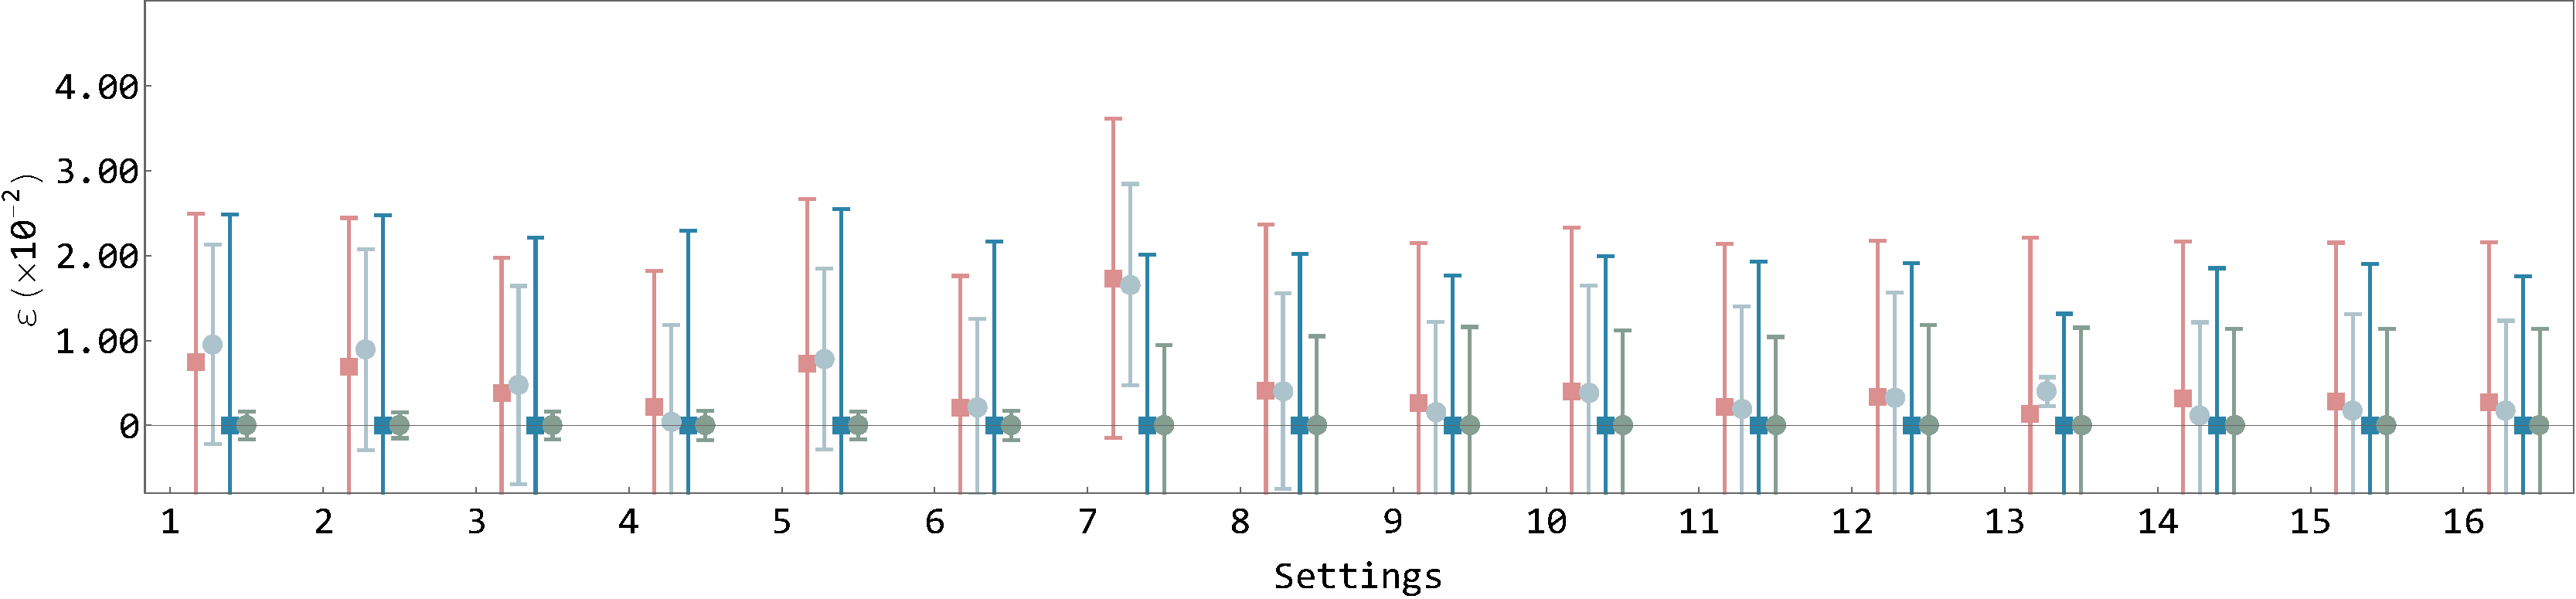
\includegraphics[width = .97 \columnwidth]{fig/exp-res-ns/1.pdf}
     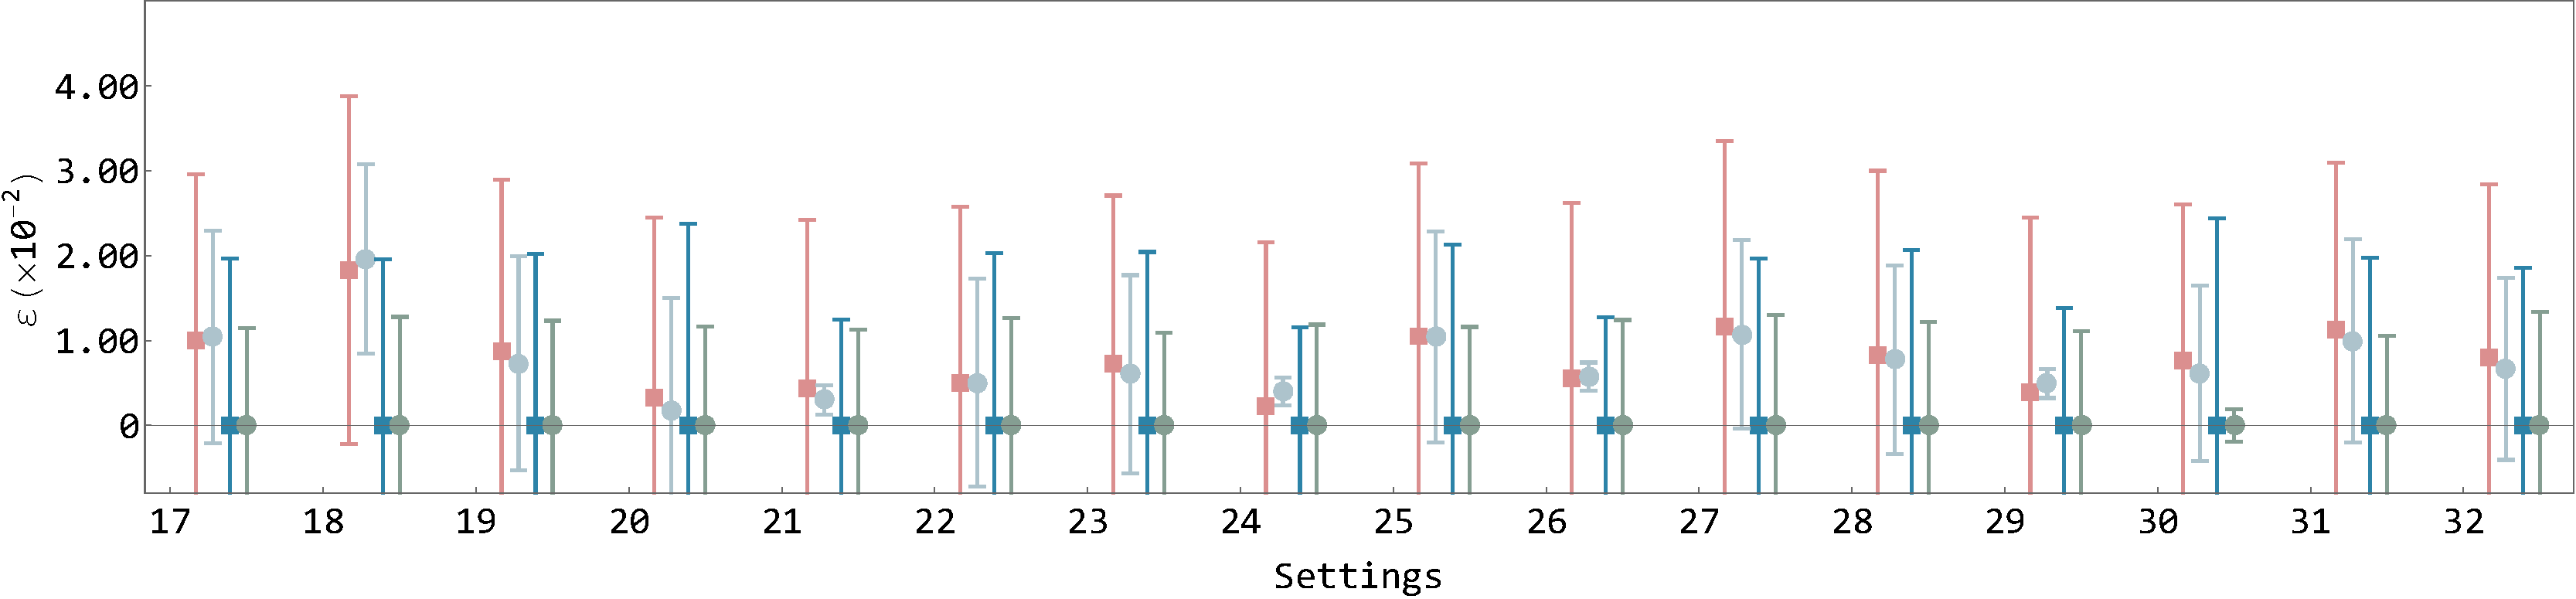
\includegraphics[width = .97 \columnwidth]{fig/exp-res-ns/2.pdf}
     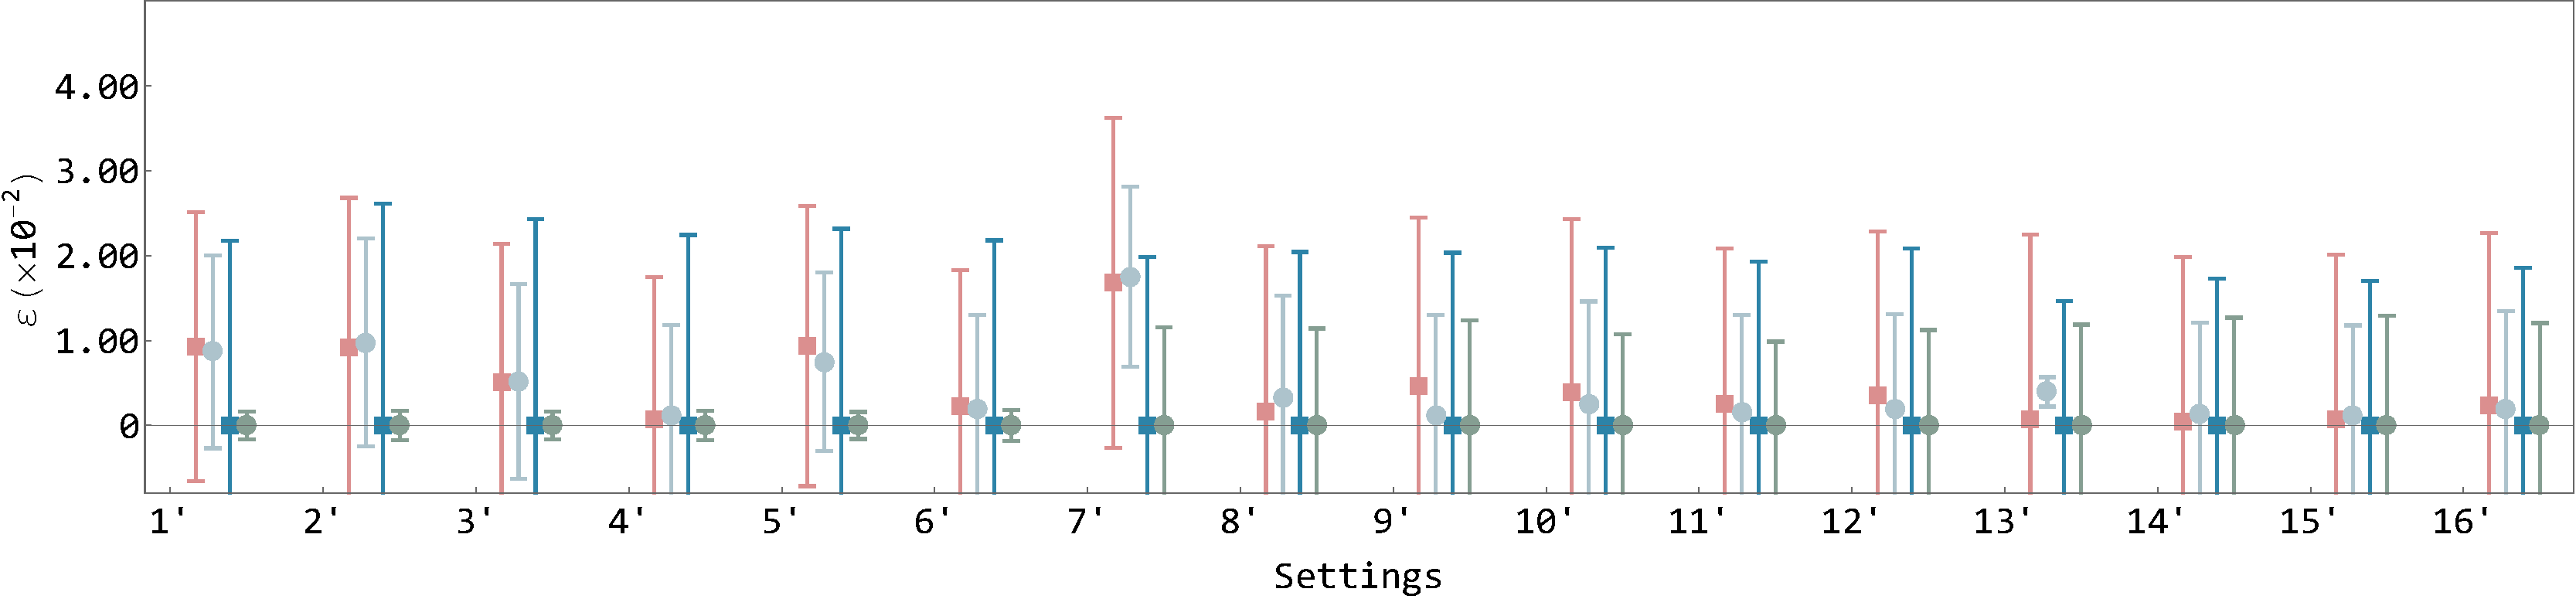
\includegraphics[width = .97 \columnwidth]{fig/exp-res-ns/3.pdf}
     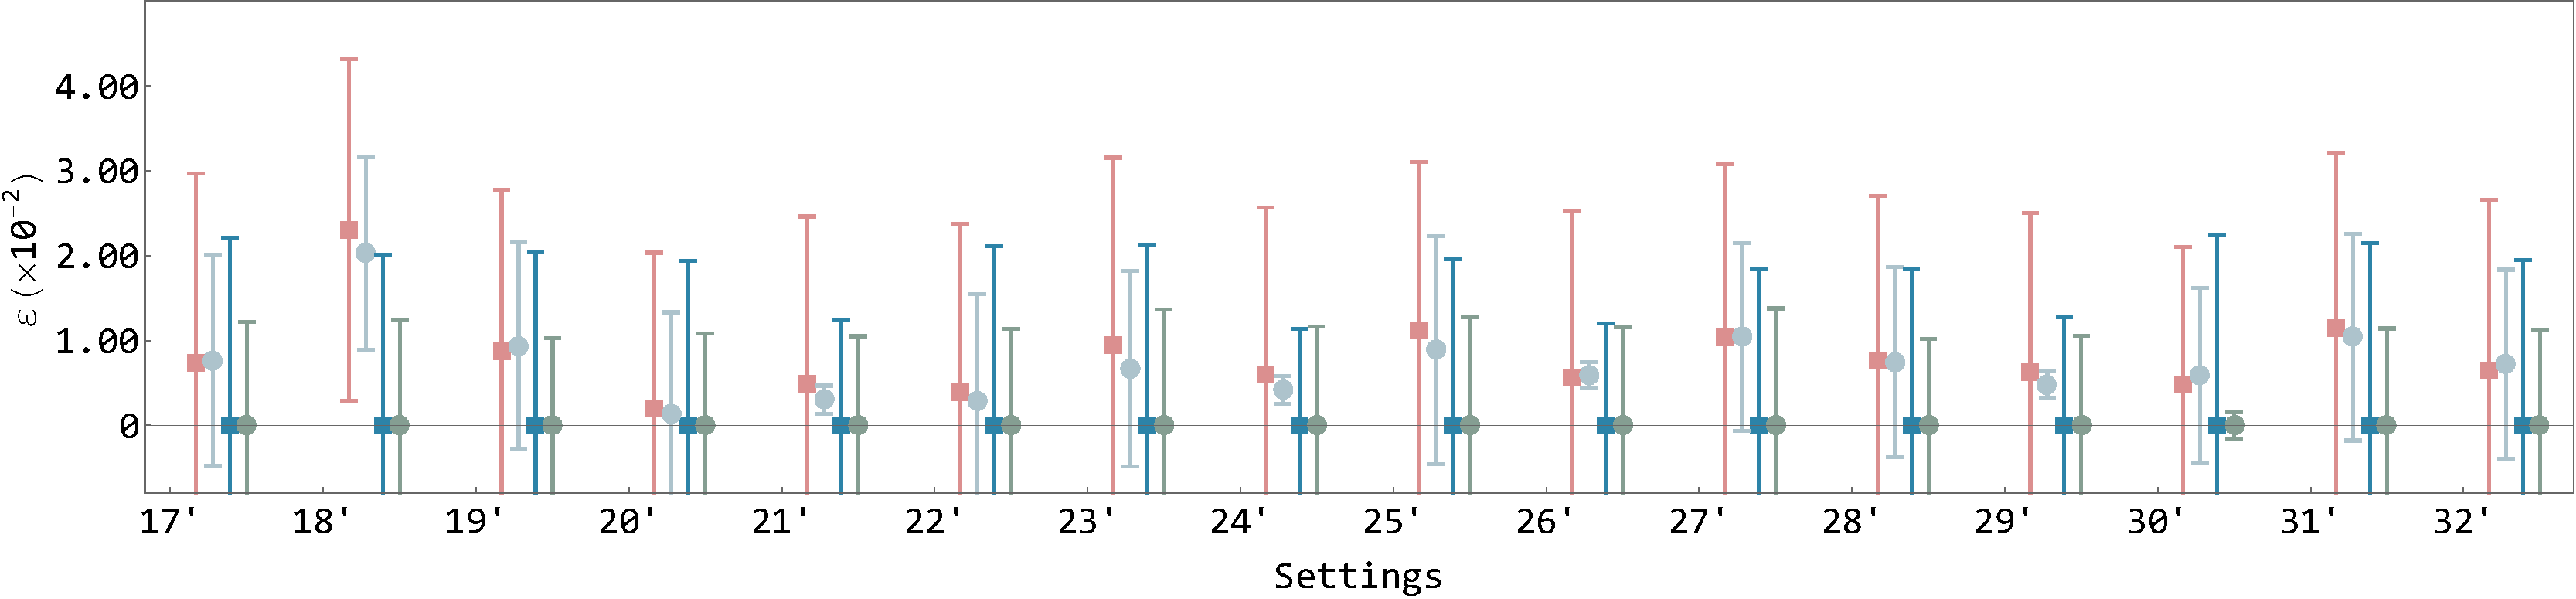
\includegraphics[width = .97 \columnwidth]{fig/exp-res-ns/4.pdf}
     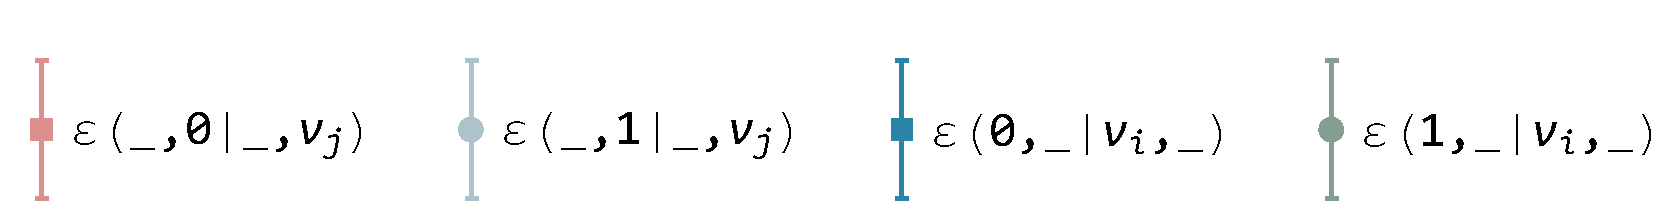
\includegraphics[width = .67 \columnwidth]{fig/exp-res-ns/0.pdf}
     \caption{Eliminating possibility of signaling between sequential measurements. By exhibiting null results for the four signaling factors $\varepsilon(0, \_|v_i, \_), \varepsilon(1, \_|v_i, \_), \varepsilon(\_, 0|\_, v_j)$ and $\varepsilon(\_, 1|\_, v_j)$, the non-signaling condition required in~\cite{cabello16s} is preserved. In each plot, the horizontal coordinate corresponds to experimental settings, i.e, different choices of states and projectors represented by edges of the exclusivity graph. The settings with primed notation swapped eigenstates and projectors. The four signaling factors are shown in four different colors.}
     \label{fig:exp-res-0}
 \end{figure}

 The key point to evaluate~(\ref{eq:averta}-\ref{eq:averte}) is to obtain $P_{\ket{\psi}} (v_i = 0, v_j = 1)$ when the task of preparing $\ket{v_i^\perp}$, the state obtained after a projective measurement of $v_i$ with outcome 0 on a system initially prepared in state $\ket{\psi}$, was encountered. In~\cite{yxiao17s}'s work, $\ket{v_i^\perp}$ was prepared by the blocking method, but this method was unlikely feasible in our setup.
 Here, we proposed a method to prepare $\ket{v_i^\perp}$ by manipulating hologram displayed on the first SLM. More precisely, the following kets were prepared,
    \begin{align}
        \widetilde{\ket{v_i^\perp}} = \ket{\psi} - \braket{v_i|\psi}\ket{v_i},
    \end{align}
 which may not be normalized as $\ket{\psi}$ and $\ket{v_i}$s would be. Rewriting~(\ref{eq:avertc}) with the notation above yields
    \begin{align}
        P_{\ket{\psi}} (v_i = 0, v_j = 1) &= P_{\widetilde{\ket{v_i^\perp}}} (v_j = 1).
    \end{align}


 From~(\ref{eq:avertd}, \ref{eq:averte}), $\varepsilon(0, \_|v_i, \_)$ and $\varepsilon(1, \_|v_i, \_)$ automatically vanish, and only the $\varepsilon(\_, 0|\_, v_j)$ and $\varepsilon(\_, 1|\_, v_j)$ terms survive. Nonetheless, the four statistical indexes are unanimously calculated.
 The result of non-signaling condition verification is shown in Fig.\ref{fig:exp-res-0}. Not all $\varepsilon(\_, 0|\_, v_j)$ and $(\_, 1|\_, v_j)$ perfectly vanish and a few error bars, which were calculated from Poisson distribution, were not guaranteed to hit zero.
 Still, the overall small absolute value of $\varepsilon$s suggested that the error was due to imperfections in state preparation and measurement and the no-signaling condition held.

\begin{thebibliography}{99}

\bibitem{BG08}
 N. Brunner and N. Gisin,
 %Partial list of bipartite Bell inequalities with four binary settings.
 \href{http://dx.doi.org/10.1016/j.physleta.2008.01.052}{Phys. Lett. A \textbf{372}, 3162 (2008).}

% \bibitem{MT} \textit{Experimental test of quantum contextuality beyond Bell nonlocality.}

\bibitem{qli18s}
 Q.~Li, et al.,
 %Experimental simulation of anti-parity-time symmetric Lorentz dynamics,
 \href{https://doi.org/10.1364/OPTICA.6.000067}{Optica \textbf{6}(1), 67 (2019).}

\bibitem{Brunner14}
 N.~Brunner, D.~Cavalcanti, S.~Pironio, V.~Scarani, and S.~Wehner,
 %Bell nonlocality,
 \href{https://doi.org/10.1103/RevModPhys.86.419}{Rev. Mod. Phys. \textbf{86} 419 (2014).}


 \bibitem{cabello16s}
 A.~Cabello,
 %Simple method for experimentally testing any form of quantum contextuality,
 \href{https://doi.org/10.1103/PhysRevA.93.032102}{Phys.~Rev.~A, \textbf{93}, 032102 (2016).}

 \bibitem{yxiao17s}
 Y.~Xiao, Z.-P.~Xu, Q.~Li, J.-S.~Xu, K.~Sun, J.-M.~Cui, Z.-Q.~Zhou, H.-Y.~Su, A.~Cabello, J.-L.~Chen, C.-F.~Li, and G.-C.~Guo,
 %Experimental observation of quantum state-independent contextuality under no-signaling conditions,
 \href{https://doi.org/10.1364/OE.26.000032}{Opt.~Express \textbf{26} 32 (2018).}


\end{thebibliography}

\end{document}


\begin{widetext}
\begin{eqnarray}\label{eqAi}
\left\{
  \begin{array}{ll}
    |\psi\rangle=[\frac{1}{\sqrt{2}},\frac{1}{\sqrt{2}},0,0],\ \ |A_1\rangle=|A_{13}\rangle=[0,0,1,0],
    \ \ |A_7\rangle=|A_{10}\rangle=[1,0,0,0],\ \ |A_9\rangle=|A_{11}\rangle=[0,1,0,0],\\
    |A_2\rangle=[\cos{[\phi_1]}\cos{[\phi_2]},\sin{[\phi_1]},0,-\cos{[\phi_1]}\sin{[\phi_2]}],\ \ |A_{16}\rangle=[\sin{[\phi_1]},\cos{[\phi_1]}\cos{[\phi_2]},0,\cos{[\phi_1]}\sin{[\phi_2]}],\\
     |A_3\rangle=[\cos{[\phi_3]},\cos{[\phi_4]}\sin{[\phi_3]},0,\sin{[\phi_3]}\sin{[\phi_4]}],\ \ |A_{5}\rangle=[\cos{[\phi_4]}\sin{[\phi_3]},\cos{[\phi_3]},0,-\sin{[\phi_3]}\sin{[\phi_4]}],\\
     |A_4\rangle=[0,\sin{[\phi_4]},0,-\cos{[\phi_4]}],\ \ |A_{8}\rangle=[\sin{[\phi_4]},0,0,-\cos{[\phi_4]}],\\
     |A_{12}\rangle=[\sin{[\phi_4]},0,0,\cos{[\phi_4]}],\ \ |A_{14}\rangle=[0,\sin{[\phi_4]},0,\cos{[\phi_4]}],\\
     |A_6\rangle=[\cos{[\phi_4]}\cos{[\phi_5]},\sin{[\phi_5]},0,\cos{[\phi_5]}\sin{[\phi_4]}],\ \    |A_{15}\rangle=[\sin{[\phi_5]},\cos{[\phi_4]}\cos{[\phi_5]},0,-\cos{[\phi_5]}\sin{[\phi_4]}],
  \end{array}
\right.
\end{eqnarray}
\end{widetext}
